
\documentclass{beamer}
\usepackage[latin1]{inputenc}
%\usetheme{Montpellier}
%\usetheme{Boadilla}
%\usecolortheme[RGB={204,51,255}]{structure}
%\usecolortheme[named=purple]{structure}
\usecolortheme[RGB={62,128,62}]{structure}
%\definecolor{dark}{rgb}{0.3,0.15,0.3}
%\definecolor{light}{rgb}{0.8,0.6,0.8}
%\definecolor{reddish}{rgb}{.5,0.15,0.15}
\definecolor{dark}{rgb}{0.5,0.3,0.4}
%\definecolor{light}{rgb}{0.8,0.6,0.8}
\definecolor{reddish}{rgb}{.7,0.25,0.25}
\definecolor{greenish}{rgb}{.25,0.7,0.25}
\definecolor{blueish}{rgb}{.25,0.25,0.7}
\definecolor{purple}{rgb}{.5,0.0,0.5}
\usepackage{graphicx}
\usepackage{pstricks}

\setbeamertemplate{navigation symbols}{}

\newcommand{\crish}{\color{reddish}}
\newcommand{\cbla}{\color{black}}
\newcommand{\cred}{\color{red}}
\newcommand{\cblu}{\color{blue}}

\usepackage{tikz}
\usetikzlibrary{arrows,decorations.markings,positioning}
\usepackage{epstopdf}

\title[Computational Neuroscience 1.2]{Computational Neuroscience 1.2}
\author{PHPH20007}
\institute{\texttt{github.com/conorhoughton/PHPH20007}}
\date{May 2019}

\begin{document}

\maketitle

\begin{frame}{The equations for a leaky bucket}
  \crish
  $$\tau\frac{dh}{dt}=\frac{1}{G}i-h$$\cbla
  
  \begin{center}
    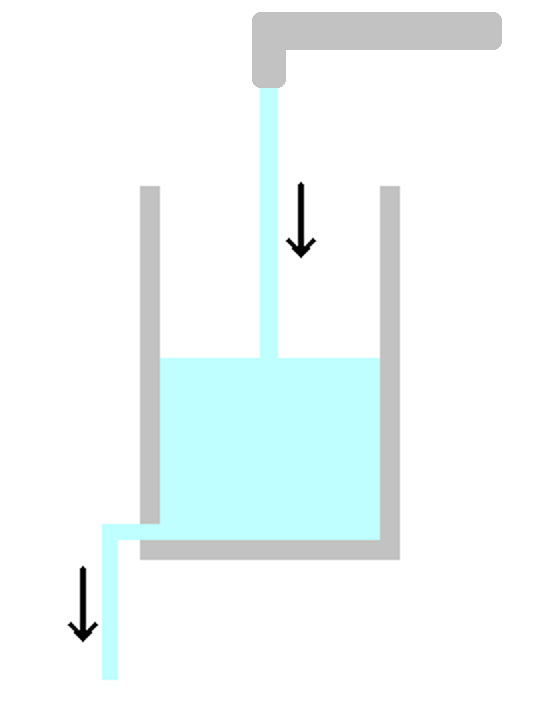
\includegraphics[height=6cm]{glass.png}
  \end{center}
\end{frame}


\begin{frame}{A neuron}
  \begin{center}
    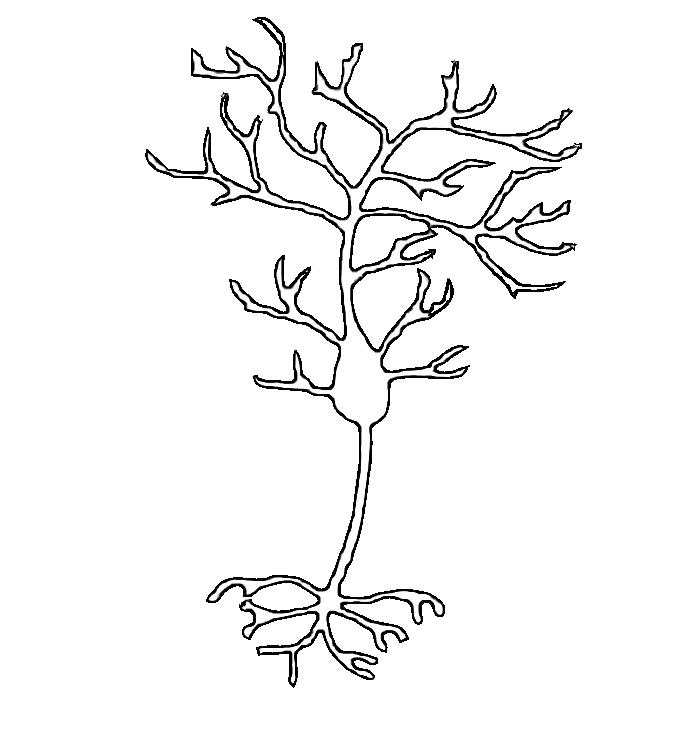
\includegraphics[height=8cm]{neuron.png}
  \end{center}
\end{frame}

\begin{frame}{A neuron has an inside and an outside}
  \begin{center}
    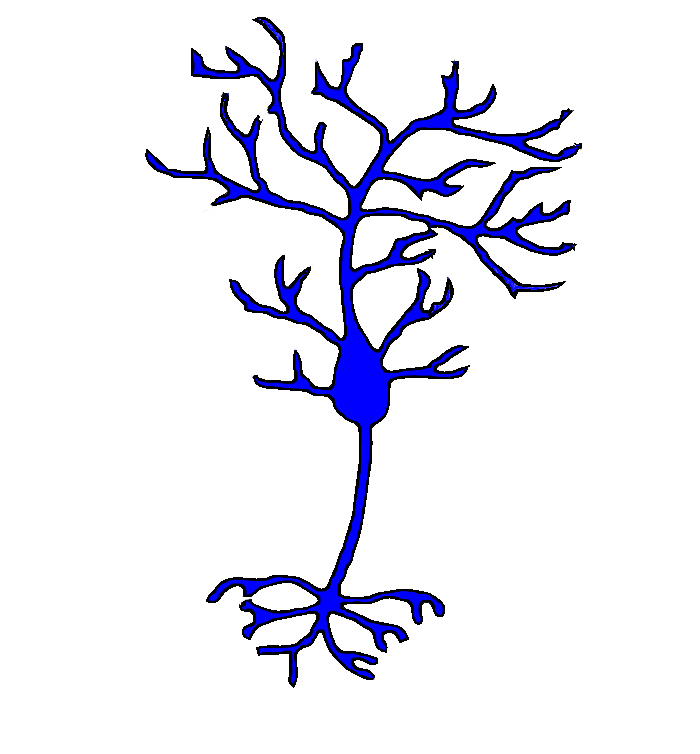
\includegraphics[height=8cm]{neuron_filled.png}
  \end{center}
\end{frame}

\begin{frame}{A neuron has an inside and an outside}
  \begin{center}
    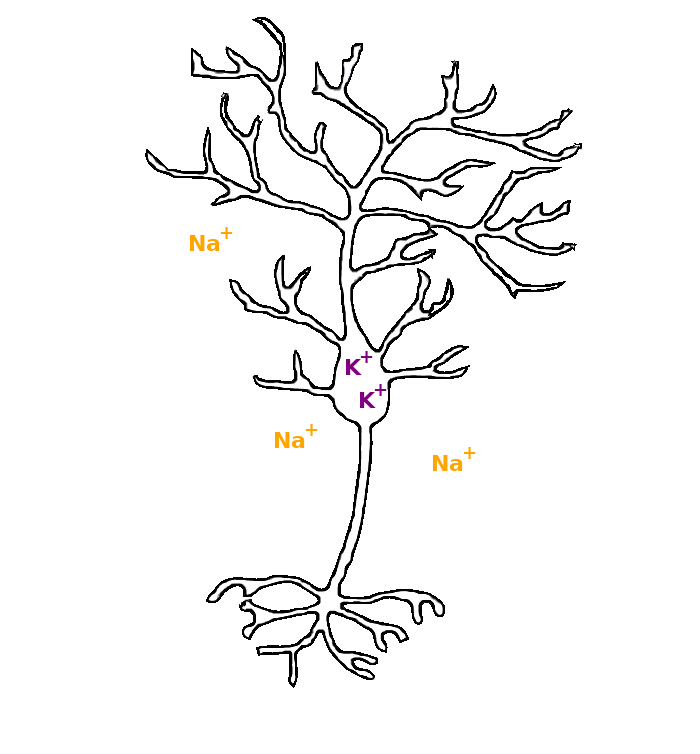
\includegraphics[height=8cm]{ions.png}
  \end{center}
\end{frame}


\begin{frame}{Ion pumps}
  \begin{center}
    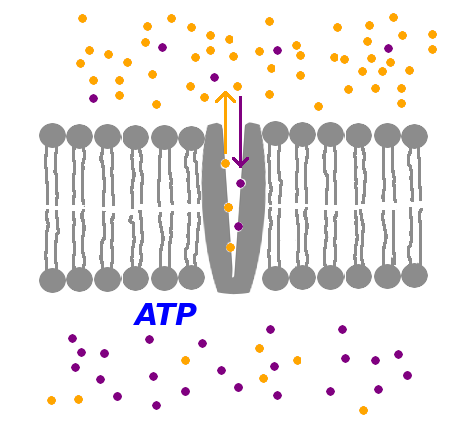
\includegraphics[height=8cm]{ion_pump_1.png}
  \end{center}
\end{frame}


\begin{frame}{Ion pumps}
  \begin{center}
    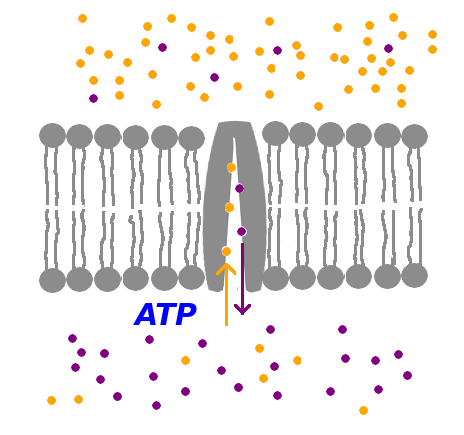
\includegraphics[height=8cm]{ion_pump_2.png}
  \end{center}
\end{frame}


\begin{frame}{Potassium inside and sodium outside}
  \begin{center}
    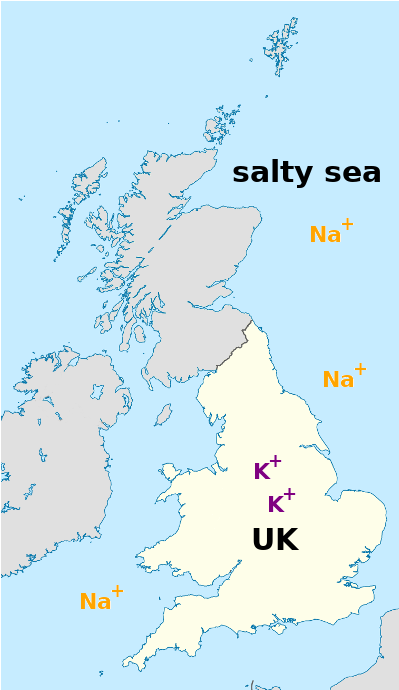
\includegraphics[height=8cm]{uk.png}
  \end{center}
\end{frame}

\begin{frame}{Ions can get through the membrane}
  \begin{center}
    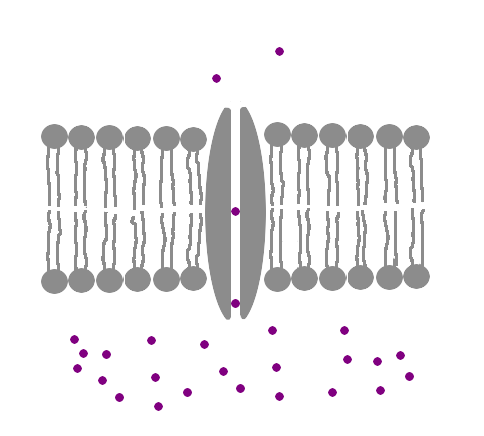
\includegraphics[height=6cm]{passive_channel.png}
  \end{center}
\end{frame}

\begin{frame}{Charge is like water}
  \begin{center}
    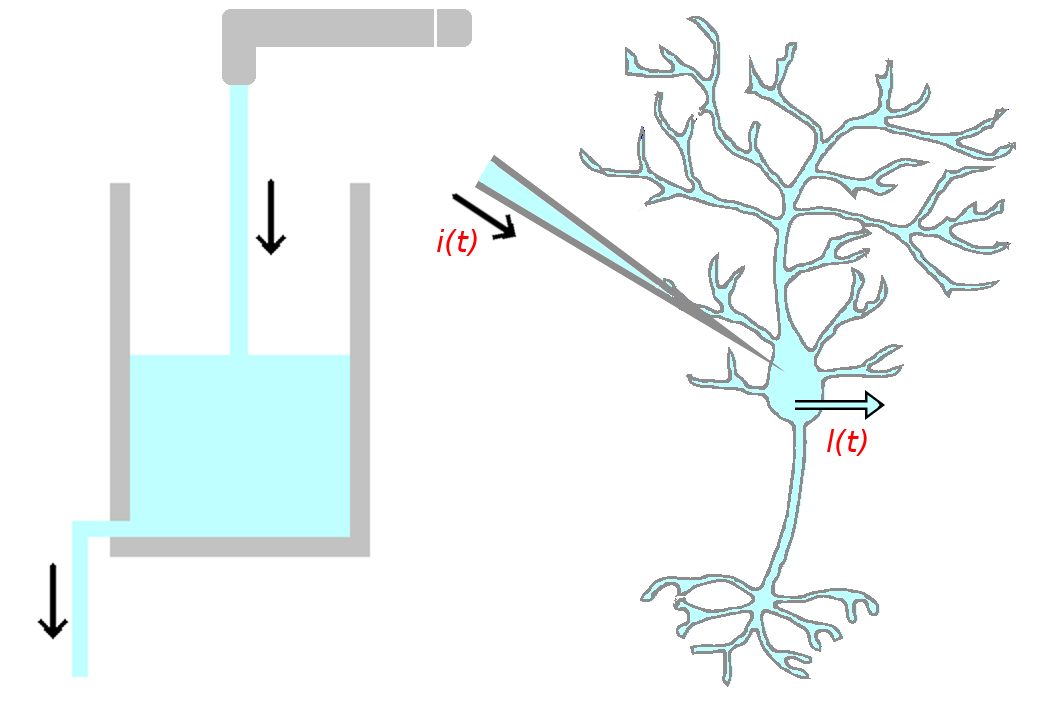
\includegraphics[height=8cm]{glass_neuron.png}
  \end{center}
\end{frame}


\begin{frame}{Voltage difference}
  \begin{columns}
        \begin{column}{0.2\textwidth}
      \end{column}
    \begin{column}{0.3\textwidth}
  $\cred V\crish\sim -70\mbox{mV}\cbla $
    \end{column}
    \begin{column}{0.3\textwidth}
    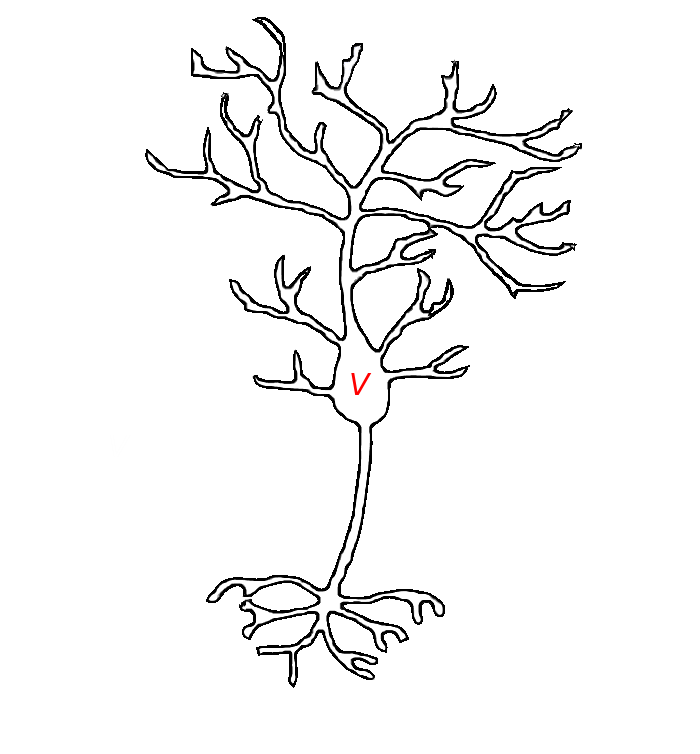
\includegraphics[height=8cm]{voltage.png}
    \end{column}
    \begin{column}{0.2\textwidth}
      \end{column}
    \end{columns}
\end{frame}

\begin{frame}{Voltage is like pressure}
  \begin{quote}
   \textbf{Voltage} is defined as the work needed per unit of charge to move a
    test charge between the two points.
  \end{quote}
\end{frame}


\begin{frame}{Capacitance}
\crish
$$Q=CV$$
\cbla  
\end{frame}


\begin{frame}{Ohm's law}
\crish
$$V=IR$$
\cbla
\begin{center}
    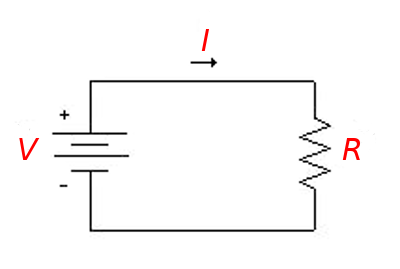
\includegraphics[height=5cm]{basic_circuit.png}
\end{center}
\end{frame}


\begin{frame}{Resistance versus Conductance}
\crish
$$G=1/R$$
\cbla{}so\crish
$$I=GV$$
\cbla
\begin{center}
    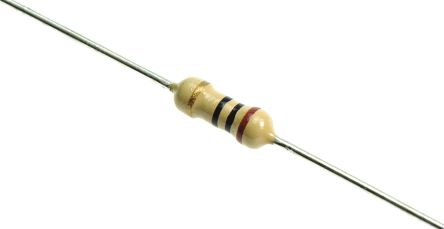
\includegraphics[height=5cm]{resistor.jpg}
\end{center}
\end{frame}


\begin{frame}{Voltage and current}
\crish
$$I=GV$$
\cbla{}so\crish{} $V=0$\cbla{} means \crish{} $I=0$\cbla{}.
\begin{center}
    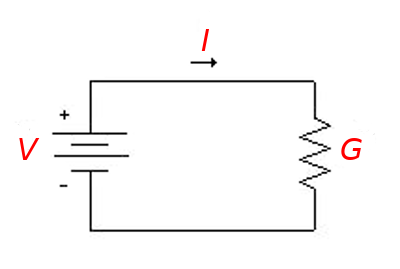
\includegraphics[height=5cm]{basic_circuit_g.png}
\end{center}
\end{frame}

\begin{frame}{Chemical gradients}
\begin{center}
    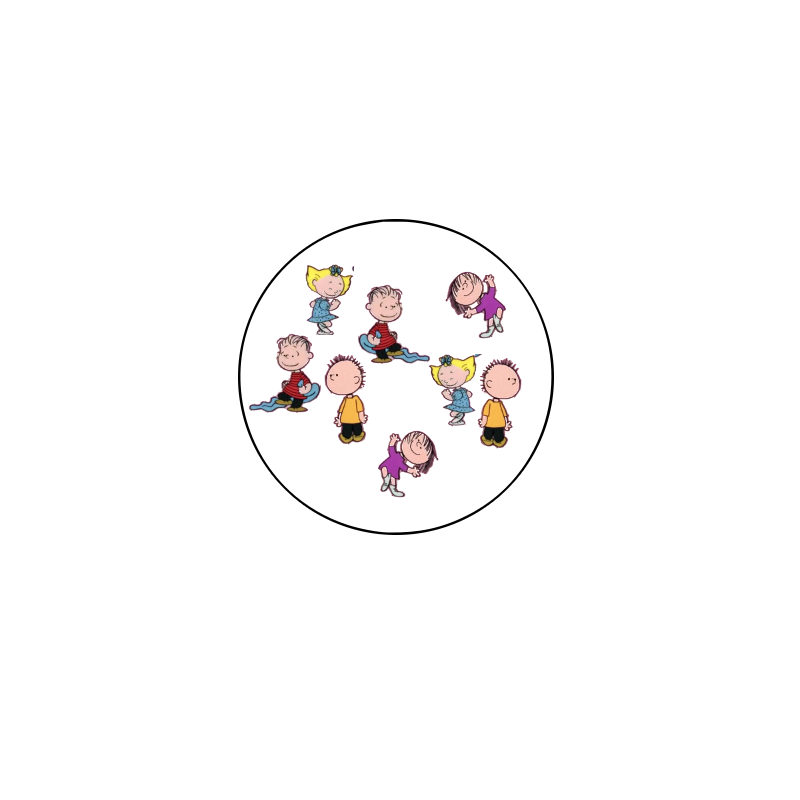
\includegraphics[height=8cm]{children1.png}
\end{center}
\end{frame}

\begin{frame}{Chemical gradients}
\begin{center}
    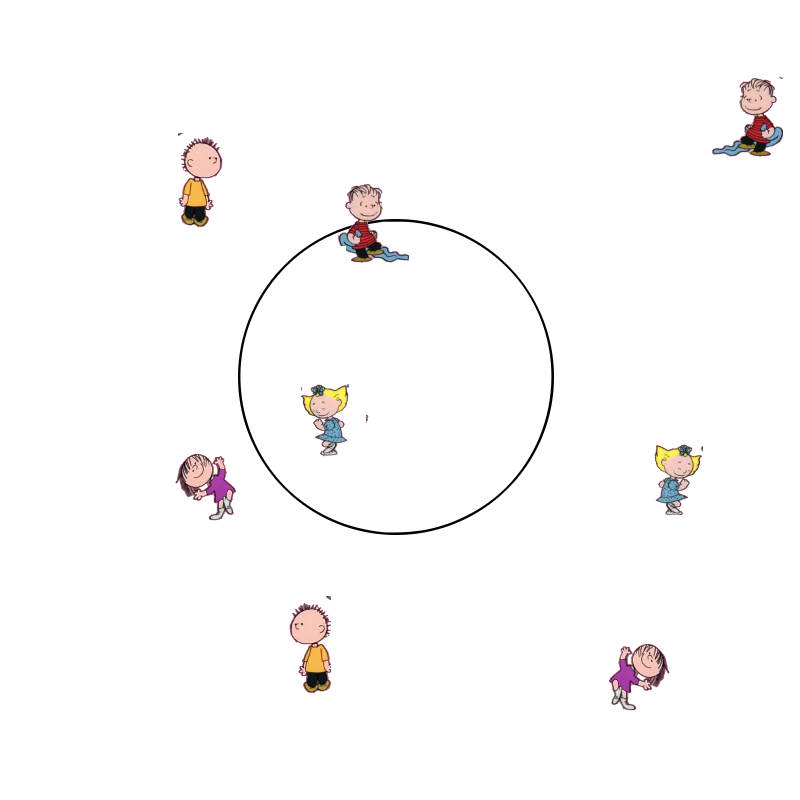
\includegraphics[height=8cm]{children2.png}
\end{center}
\end{frame}

\begin{frame}{Chemical gradients}
\begin{center}
    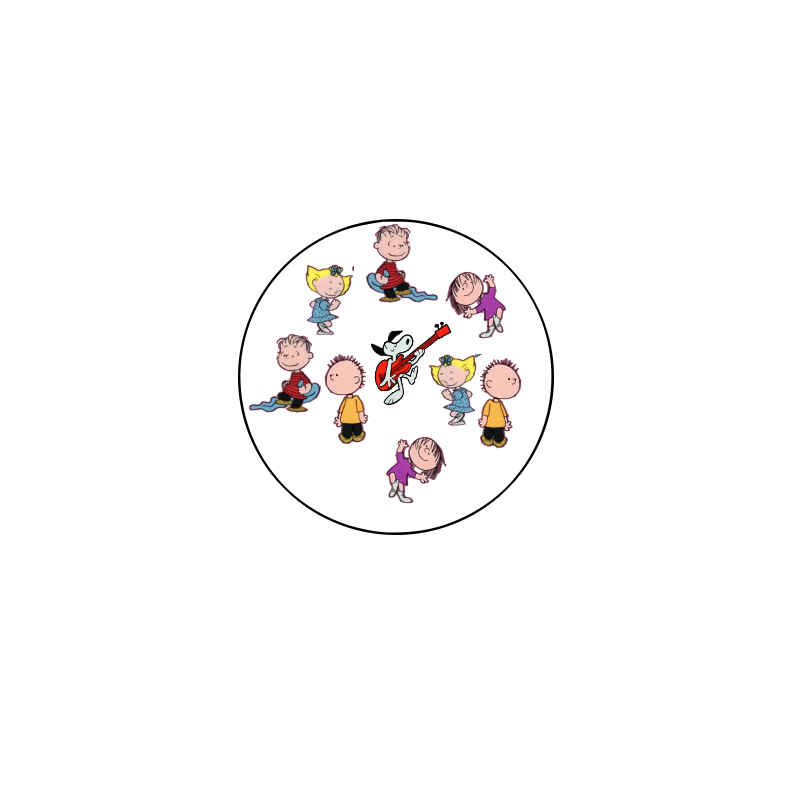
\includegraphics[height=8cm]{children3.png}
\end{center}
\end{frame}

\begin{frame}{Chemical gradients}
\begin{center}
    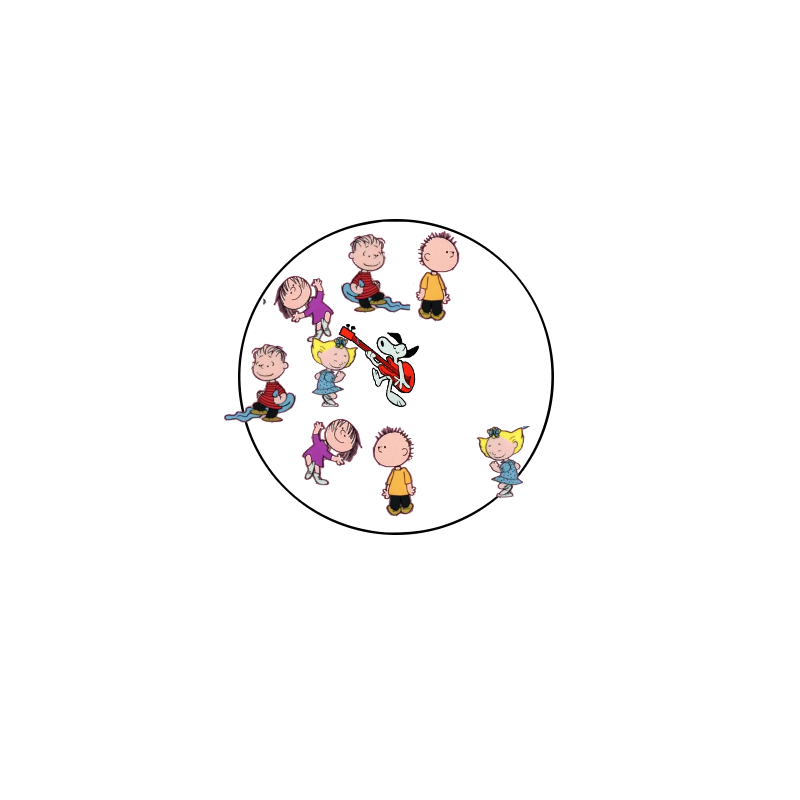
\includegraphics[height=8cm]{children4.png}
\end{center}
\end{frame}

\begin{frame}{Chemical gradients}
  \begin{center}
    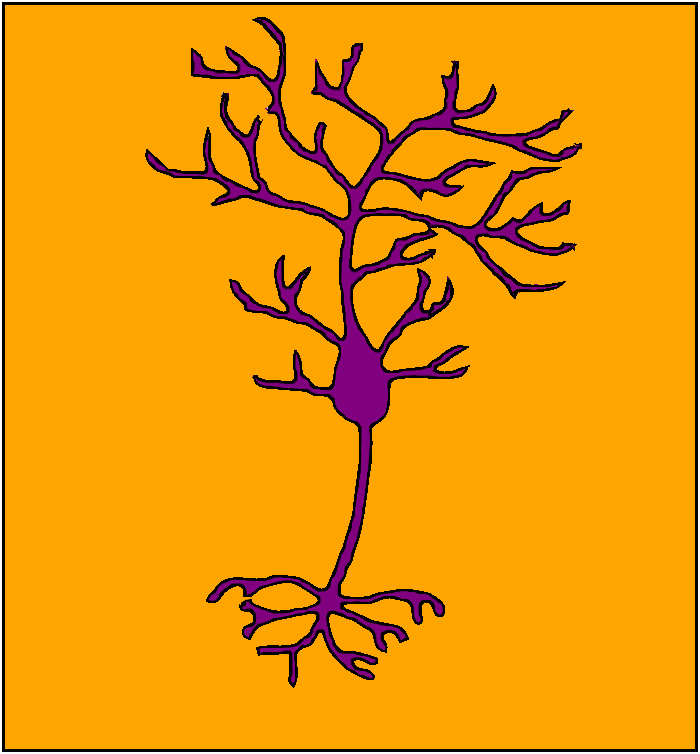
\includegraphics[height=8cm]{neuron_ions.png}
  \end{center}
\end{frame}


\begin{frame}{Chemical gradients}
  \begin{center}
    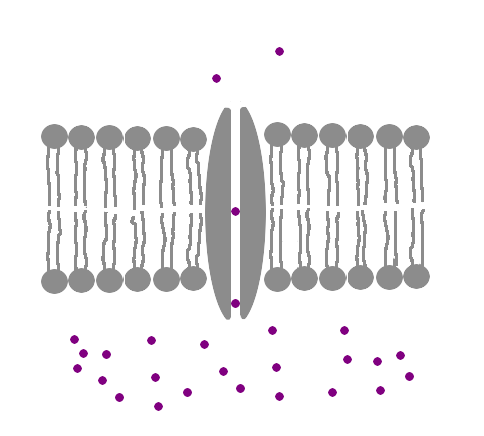
\includegraphics[height=6cm]{passive_channel.png}
  \end{center}
\end{frame}


\begin{frame}{Leak potential}
  \crish
  $$I=G(\cred{}E_l\crish{}-V)$$
\cbla{}
  where \cred$E_l\sim -70$mV\cbla{} is the \cblu{}leak reversal potential\cbla{}. 
\end{frame}


\begin{frame}{Leak potential}
  \crish
  $$I=G(\cred{}E_l\crish{}-V)$$
\cbla{}

DON'T WORRY TO MUCH ABOUT THE SIGN, it is easy to get confused so I
WILL MAKE SURE IT IS RIGHT, this is the expression for the current
inward.
\end{frame}



\begin{frame}{Leak conductance}
  \crish
  $$I=\cred{}G\crish{}(E_l-V)$$

  \cbla{} The conductance \cred$G$\cbla{} is the conductance of the membrane and is often called the \cblu{}leak conductance\cbla{}, in fact, there are other conductance that depend on \crish$V$\cbla{}, whereas the leak conductance is constant and sometimes called \cblu{}passive\cbla{}. The symbol \cred{}$g_l$\cbla{} is often used:

  \crish
  $$I=g_l(E_l-V)$$
\cbla{}
\end{frame}

\begin{frame}{The leaky integrator for neurons}
\begin{quote}
  rate of change of charge = current in - leak out
\end{quote}
\end{frame}

\begin{frame}{The leaky integrator for neurons}
  \crish
  $$\frac{dQ}{dt}=i(t)-l(t)$$
  \cbla
\end{frame}

\begin{frame}{Input}
  For now imagine the input is from an electrode, the electrode input is written:\crish
  $$i(t)=I_e(t)$$
  \cbla
\end{frame}

\begin{frame}{The leaky integrator for neurons}
  \crish
  $$C\frac{dV}{dt}=g_l(E_l-V)+I_e(t)$$
  \cbla
\end{frame}


\begin{frame}{The leaky integrator for neurons}
Dividing across by the \crish{}$g_l$\cbla{} we get
  \crish
  $$\tau_m\frac{dV}{dt}=E_l-V+R_mI_e(t)$$
  \cbla
  where \crish$\tau_m$\cbla{} is called the \cblu{}membrane time constant\cbla{} and \crish{}$R_m=1/g_l$\cbla{} is called the \cblu{}the membrane resistance\cbla{}.

\end{frame}



\begin{frame}{The leaky bucket redux}

  \crish
  $$\tau_m\frac{dV}{dt}=E_l-V+R_mI_e(t)$$
  \cbla

  We have seen more-or-less this equation before, all that is really
  different is the extra constant \crish$E_l$\cbla{} and so know how to
  deal with the equation, for example, if \crish{}$I_e$\cbla{} is constant the
  solution is\crish

  $$V(t)=E_l+R_mI_e+[V(0)-E_l-R_mI_e]e^{-t/\tau_m}$$
  \cbla{}
  
\end{frame}

\begin{frame}{Voltage gated channels}
  This isn't the full story
  \crish$$\tau_m\frac{dV}{dt}=E_l-V+R_mI_e(t)+R_m(\cblu{}\mbox{currents from the gated channels}\crish)$$\cbla{}
  \begin{center}
    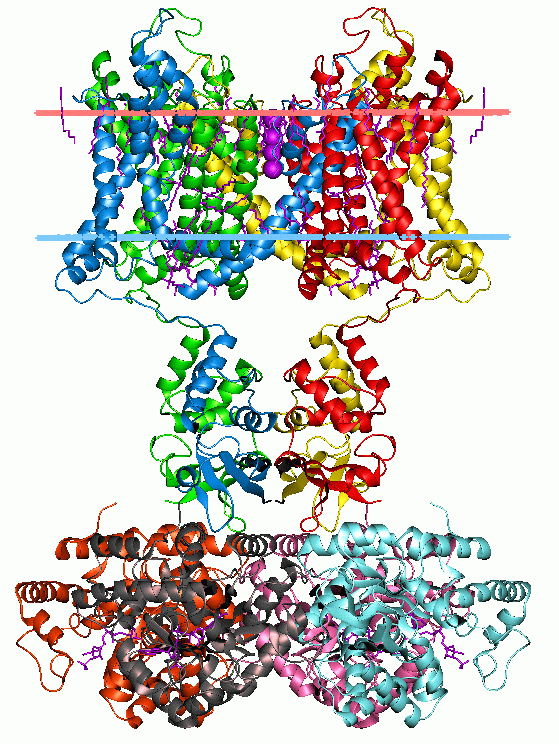
\includegraphics[height=5cm]{2r9r_opm.png}
\end{center}
    \vfill
  \flushright{\tiny{image from wikipedia}}
  \end{frame}


\end{document}

